\documentclass[tikz, convert]{standalone}

\begin{document}
    
    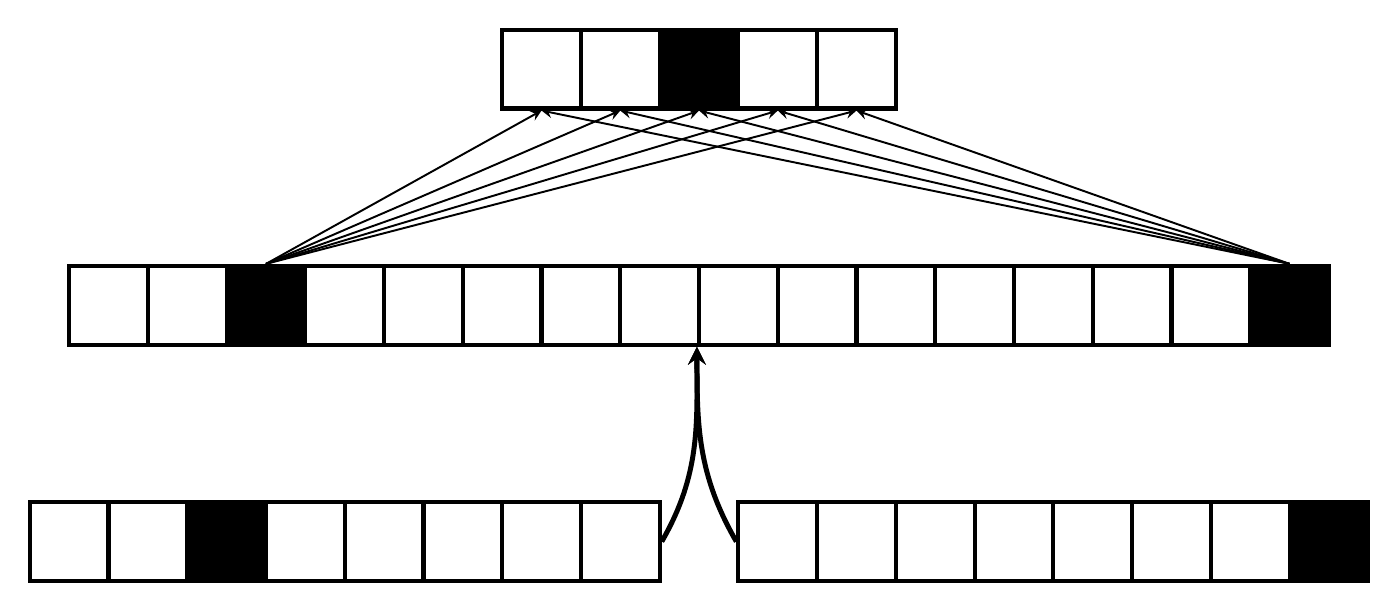
\begin{tikzpicture}[->, >=stealth, every node/.style={rectangle, line width=1.5pt, draw, minimum width=1cm, minimum height=1cm, font=\bfseries}]
    \label{logistic_regression}
        
        % First input.
        \foreach \x in {-8,...,-1}
            \node (I_1-\x) at (\x,0) {};
        \node[fill=black] (I_1--6) at (-6,0) {};
        
        % Second input.
        \foreach \x in {1,...,8}
            \node (I_2-\x) at (\x,0) {};
        \node[fill=black] (I_2-8) at (8,0) {};
        
        % Concatenate.
        \foreach \x in {-8,...,7}
            \node[xshift=0.5cm] (C-\x) at (\x,3) {};
        \node[xshift=0.5cm,fill=black] (C--6) at (-6,3) {};
        \node[xshift=0.5cm,fill=black] (C-7) at (7,3) {};
        
        \path[->, line width=1.8pt] (I_1--1.east) edge [out=60, in=270] (C-0.south west);
        \path[->, line width=1.8pt] (I_2-1.west) edge [out=120, in=270] (C-0.south west);
        
        % Output.
        \foreach \x in {-2,...,2}
            \node (O-\x) at (\x,6) {};
        \node[fill=black] (O-0) at (0,6) {};
        
        % Batter connections.
        \foreach \dest in {-2,...,2}
            \path[line width=0.7pt] (C--6.north) edge (O-\dest.south);
        
        % Pitcher connections.
        \foreach \dest in {-2,...,2}
            \path[line width=0.7pt] (C-7.north) edge (O-\dest.south);
        
    \end{tikzpicture}

\end{document}